
%
% state - drupal mapping
%

\section{Drupal \& Mapping}
\label{chapter:drupal-mapping}

The book ``Mapping with Drupal''~\cite{Zzolo11mappingdrupal} by Alan Palazzolo and Thomas Turnbull was published at the end of 2011 and gives a throughout overview of available mapping modules for Drupal 7 by that time. As the web, Drupal is a constantly evolving platform. Development continues, so its a permanent exercise to keep up-to-date with recent technologies.

\subsection{Drupal}

Drupal is a free and open source content management system and framework\footnote{\url{http://drupal.org}}. Developed and maintained by an international community, it currently backs more than 2\% of all websites worldwide. It is used to create personal blogs, corporate and government sites and is also used as knowledge management and business collaboration tool\cite{wiki:drupal}.

Drupal is a set of PHP scripts that can be extended by using existing and creating custom modules. It is beyond the scope of this thesis to explain Drupal in detail, but the following terms will be used throughout this thesis:

\begin{itemize}

\item \textbf{hooks}: while using APIs and object-oriented programming are familiar concepts, \textit{hooks} are a Drupal-specific concept. They basically allow modules to interact with each other in a procedural way in which many parts of the Drupal system are built.

\begin{quote}
Drupal's module system is based on the concept of "hooks". A hook is a PHP function that is named foo\_bar(), where "foo" is the name of the module (whose filename is thus foo.module) and "bar" is the name of the hook. Each hook has a defined set of parameters and a specified result type.

To extend Drupal, a module need simply implement a hook. When Drupal wishes to allow intervention from modules, it determines which modules implement a hook and calls that hook in all enabled modules that implement it.\footnote{\url{http://api.drupal.org/api/drupal/includes!module.inc/group/hooks/7}}
\end{quote}

\item \textbf{Entities and Fields}: Since Drupal 7, the generic concept of \textit{entities} provides content and data containers which are used in Drupal to represent content like \textit{nodes} but also \textit{users}, \textit{comments}, etc. \textit{Fields} empower site builders to assign fields to various entity types which allows for a flexible content modeling framework\cite{klausi-thesis}.

\item \textbf{patches}: the term \textit{patch} describes a way to submit code changes used within the Drupal and other open source communities:

\begin{quote}
Patches are pieces of code that solve an existing issue. In fact, patches describe the changes between a before and after state of either a module or core. By applying the patch the issue should no longer exist.

Patches are used to maintain control-ability over the entire Drupal project. While Drupal is distributed via the git version control system, patches are additional pieces of code that focus on a single change request and therefore are easily tested, reviewed and documented.\footnote{\url{http://drupal.org/patch}}
\end{quote}

\end{itemize}

In the following, mapping-related technologies for Drupal 7 are explained. 

\subsection{Data storage}

The \textbf{Geofield}\footnote{\url{http://drupal.org/project/geofield}} module is stated to be the ``best choice for all but the simplest mapping applications''~\cite[page 27]{Zzolo11mappingdrupal} in Drupal 7. It is based on the concept of \textit{Entities} and \textit{Fields} that has been introduced in the previous section. By using the \textit{geoPHP library}\footnote{\url{https://github.com/phayes/geoPHP}} for geometry operations, it allows to store location data in various formats as latitude/longitude, WKT. Geofield integrates with various other mapping modules related to data input and storage in Drupal, as illustrated in figure \ref{fig:geofield}.

\begin{figure}[h]
  \begin{center}
    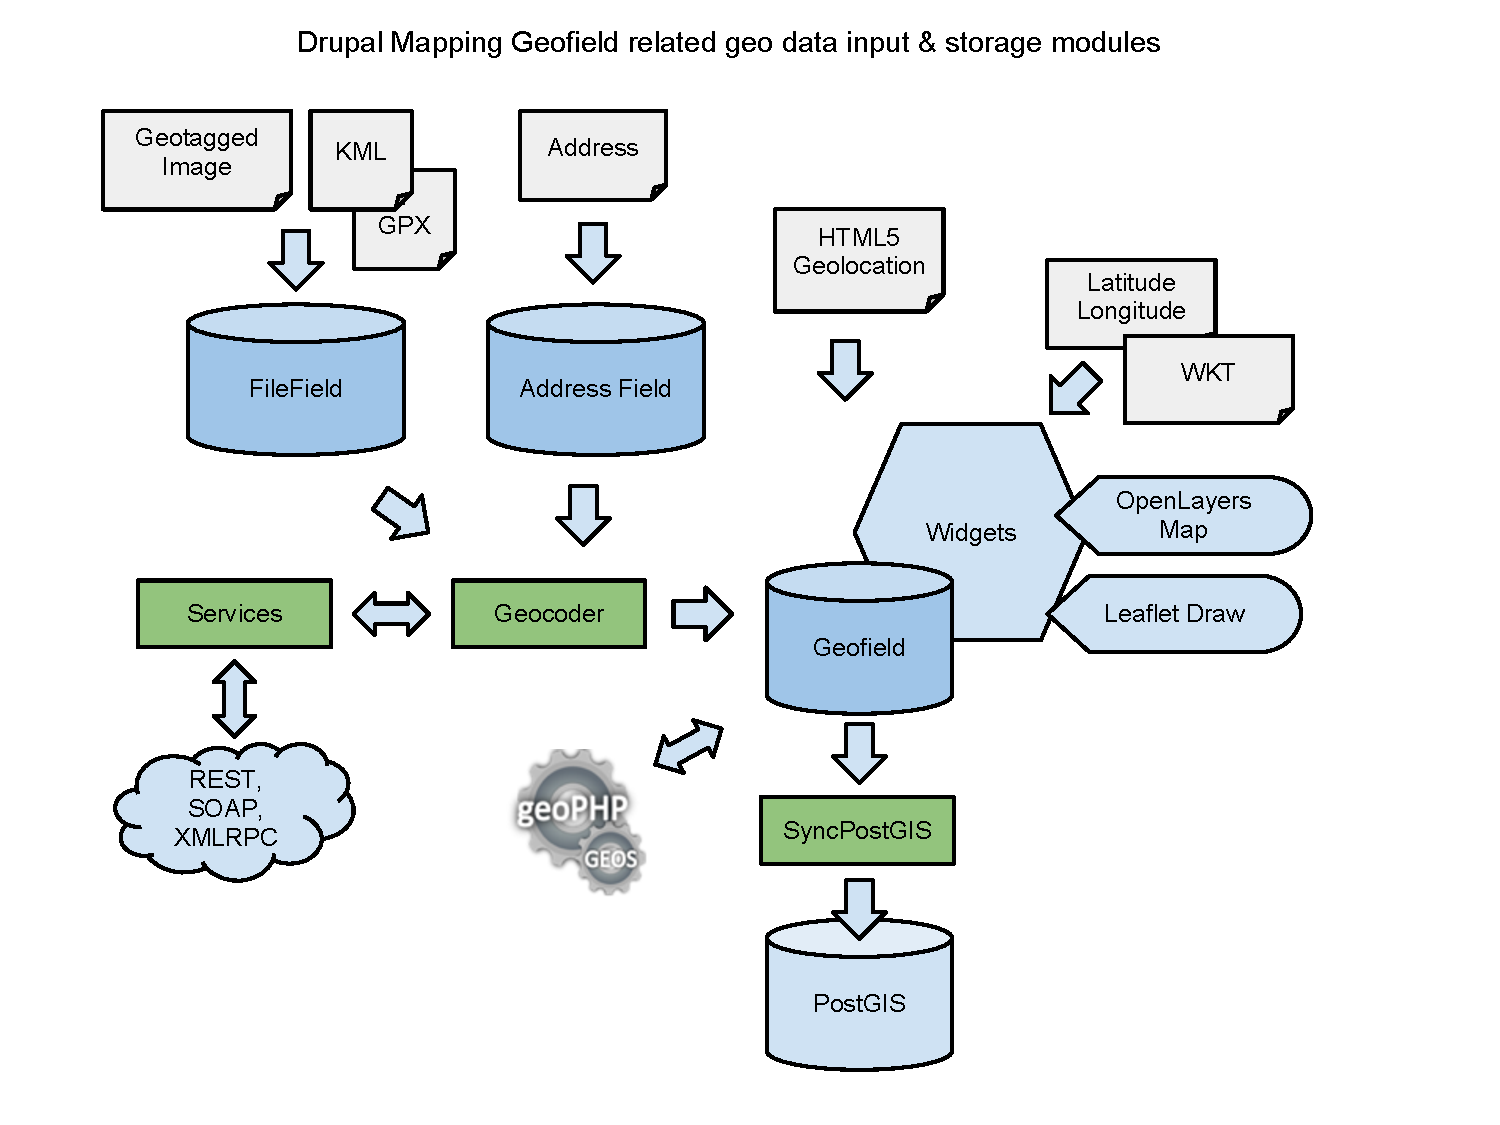
\includegraphics[width=1.2\textwidth]{figures/drupal_mapping_geofield.pdf}
    \caption{The Drupal Geofield module and related geo data input and storage modules.}
    \label{fig:geofield}
  \end{center}
\end{figure}

Besides the Geofield module, the following modules are relevant when considering ways to store location data in Drupal: 

\begin{itemize}

\item \textbf{PostGIS integration} is often requested when dealing with complex spatial data. A variety of modules and approaches exist for integration with PostGIS. The \textit{PostGIS} module\footnote{\url{http://drupal.org/project/postgis}} is similar to Geofield, but relies on PostGIS for spatial operations and data storage. \textit{Sync PostGIS}\footnote{\url{http://drupal.org/project/sync_postgis}} allows to push geospatial data from a Drupal-internal storage as Geofield into PostGIS. Recently, a pluggable storage backend was added\footnote{\url{http://drupal.org/node/1728530}} to the Geofield module in order to allow integration with alternative databases. \textit{Geofield PostGIS}\footnote{\url{https://github.com/phayes/geofield_postgis}} therefore is a more integrated option for storing Geofield data in PostGIS.

\item \textbf{Solr integration} is another common approach when creating maps based on Drupal. \textit{Apache Solr search} is a fast open source search platform written in the Java programming language. There are two common modules for Solr integration in Drupal, which both offer support for indexing spatial data: \textit{Search API}\footnote{\url{http://drupal.org/project/search_api}} and \textit{Apache Solr Search Integration}\footnote{\url{http://drupal.org/project/apachesolr}}.

\item The \textbf{Location}\footnote{\url{http://drupal.org/project/location}} module is another popular choice for storing spatial data in Drupal 7. As its architecture doesn't follow current Drupal conventions, its rather a monolithic system that provides a rich out-of-the-box experience but doesn't integrate that well with other modules like Geofield does~\cite{Zzolo11mappingdrupal}.

\end{itemize}

\subsection{Data presentation}

Being a content management system and framework, the second most important task for handling spatial data in Drupal is presenting it in various ways. Again, a variety of modules exists for querying and displaying geospatial data. Figure \ref{fig:drupal-mapping-display} illustrates how the query- and display-related Drupal mapping modules work together in a common use case.

A \textbf{mapping module} provides the basic integration for a JavaScript mapping library with the Drupal internals. The most widely used mapping modules are the \textit{OpenLayers} module\footnote{\url{http://drupal.org/project/openlayers}} with 8,325 active installations on Drupal 7 by April 2013 and the GMap module\footnote{\url{http://drupal.org/project/gmap}} with 24,113. The Leaflet module\footnote{\url{http://drupal.org/project/leaflet}} only counts 838 active installations reported on drupal.org by that time, but has the advantage of being more lightweight than OpenLayers and is not bound to a single, commercial API such as GMap.

\begin{figure}[h]
  \begin{center}
    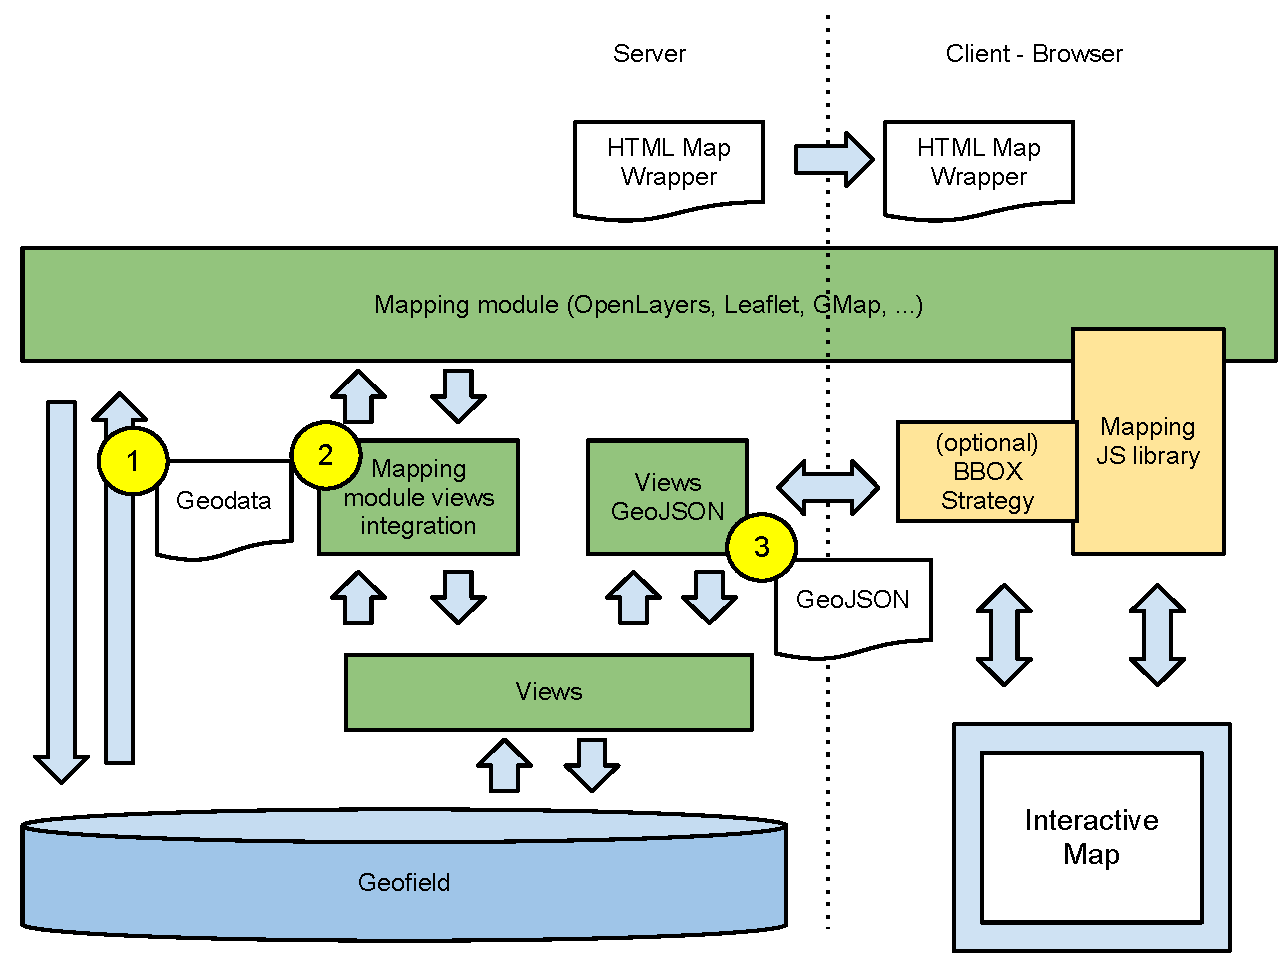
\includegraphics[width=1\textwidth]{figures/drupal_mapping_display.pdf}
    \caption{The prototypic work-flow of query and display-related Drupal mapping modules.}
    \label{fig:drupal-mapping-display}
  \end{center}
\end{figure}

The interaction with the spatial data provided by the Geofield module can be classified into three different scenario types, visualized by circles within figure \ref{fig:drupal-mapping-display}:

\begin{enumerate}

\item In the first scenario, the mapping module directly accesses data from Geofield.

This approach is usually applied when displaying maps for single single pieces of content with location. The geo data retrieved from Geofield is then transferred to the client within the HTML response. On the client-side, the JavaScript mapping library takes care of visualizing the geo data.

\item In the second scenario, integration with the \textbf{Views} module is used to query a collection of data.

The Drupal \textit{Views} module\footnote{\url{http://drupal.org/project/views}} is the de-facto standard for creating listings of content of any kind. With 422,100 reported installations in Drupal 7 by April 2013, it is the most widely used module and it also will be part of Drupal 8 core. This powerful tool allows site builders to configure database queries using an administration interface. In addition, the module provides formatting options for representing query results. In combination with extension modules, Views allows to create lists, tables and many other formats based on a collection of dynamic data. Using Views allows the mapping module to query a listing of locations from Geofield, based on user-defined parameters. Instead of returning single locations as in scenario one, the second therefore processes a collection of geo data values.

\item Scenario three allows for dynamically updating the map based on user interaction.

In this case, the geospatial data is not delivered within the HTML response, as in the previous approaches. The JavaScript library issues a separate request to the server using a \textbf{Bounding Box strategy}. The OpenLayers JavaScript library contains such a BBOX Strategy\footnote{\url{http://dev.openlayers.org/docs/files/OpenLayers/Strategy/BBOX-js.html}} and the \textit{Leaflet GeoJSON} module\footnote{\url{http://drupal.org/project/leaflet_geojson}} provides the same for the Leaflet library. The strategy essentially requests the geo data within the bounding box of the current viewport. On the server-side, the \textit{Views GeoJSON} module\footnote{\url{http://drupal.org/project/views_geojson}} initiates the query and transforms the data returned by Views into a \textit{GeoJSON}\footnote{\url{http://www.geojson.org/}} feed in order to deliver it to the JavaScript mapping library on the client-side.

\end{enumerate}

Note, that the exact implementation details vary between the used mapping modules.

\textbf{Solr integration} for querying and displaying geospatial data in Drupal is mainly provided by the integration of the Solr-related modules with Views. For the \textit{Apache Solr Search Integration} module exists a \textit{apachesolr\_location} module\footnote{\url{http://drupal.org/project/apachesolr_location}} and a \textit{ApacheSolr Geo} sandbox project\footnote{\url{http://drupal.org/sandbox/pwolanin/1497066}}. For \textit{Search API} there is a \textit{Search API Location}\footnote{\url{http://drupal.org/project/search_api_location}} module.




